% =========================================================================
% Chapter 5: Results
% =========================================================================

\chapter{Results}
\label{ch:results}

\section{Aqueous extract}
\label{sec:results_yield}

The recorded crude yield of the aqueous extract was 24.13\% (w/w). That mass is larger than the dichloromethane (2.72\%) and methanol (2.9\%) yields reported by \citet{drakhshaan2026} for the same species. Water co-extracts sugars, mucilage, and glycosides as well as phenolics, so a larger crude mass does not by itself mean a richer antibacterial fraction.

\section{Qualitative phytochemistry}
\label{sec:results_phytochem}

All nine classes screened were recorded as positive (\autoref{tab:phytochem_results}; \autoref{fig:phytochem}). The tests are presence/absence colour reactions. They do not quantify rutin, ferulic acid, or any other marker reported from organic-solvent extracts of this species \citep{drakhshaan2026}.

\begin{table}[htbp]
  \centering
  \caption{Qualitative phytochemical profile of the aqueous extract ($+$ = detected).}
  \label{tab:phytochem_results}
  \begin{tabular}{lc}
    \toprule
    \textbf{Constituent} & \textbf{Result} \\
    \midrule
    Flavonoids & $+$ \\
    Phenolics & $+$ \\
    Quinones & $+$ \\
    Terpenoids & $+$ \\
    Tannins & $+$ \\
    Carbohydrates & $+$ \\
    Saponins & $+$ \\
    Alkaloids & $+$ \\
    Phytosterols & $+$ \\
    \bottomrule
  \end{tabular}
\end{table}

\section{Zone of inhibition: \textit{Escherichia coli}}
\label{subsec:results_ecoli}

Against \textit{E.\ coli}, mean zone diameter increased from C1 to C2 (\autoref{tab:zoi_ecoli}). The distilled-water control gave 0.00\,mm. The gentamicin disc gave \qty{17.00 \pm 0.00}{\milli\metre}. A representative plate is \autoref{fig:ecoli_inhibition}; lid marks distinguish N (negative) from C (extract) but do not label C1 versus C2.

\begin{table}[hbt!]
  \centering
  \caption{Zone of inhibition (mm), inclusive of the disc, of aqueous \textit{D.\ inermis} against \textit{Escherichia coli} (mean $\pm$ SD, $n = 3$). C1 = \qty{50}{\milli\gram\per\milli\litre}; C2 = \qty{100}{\milli\gram\per\milli\litre}.}
  \label{tab:zoi_ecoli}
  \begin{tabular}{lcccc}
    \toprule
    Treatment & R1 & R2 & R3 & Mean $\pm$ SD \\
    \midrule
    C1 & 12.00 & 11.78 & 12.05 & $11.94 \pm 0.14$ \\
    C2 & 15.00 & 15.50 & 14.48 & $14.99 \pm 0.51$ \\
    Gentamicin disc ($+$) & 17.00 & 17.00 & 17.00 & $17.00 \pm 0.00$ \\
    Distilled water ($-$) & 0.00 & 0.00 & 0.00 & $0.00 \pm 0.00$ \\
    \bottomrule
  \end{tabular}
\end{table}

\begin{figure}[htbp]
  \centering
  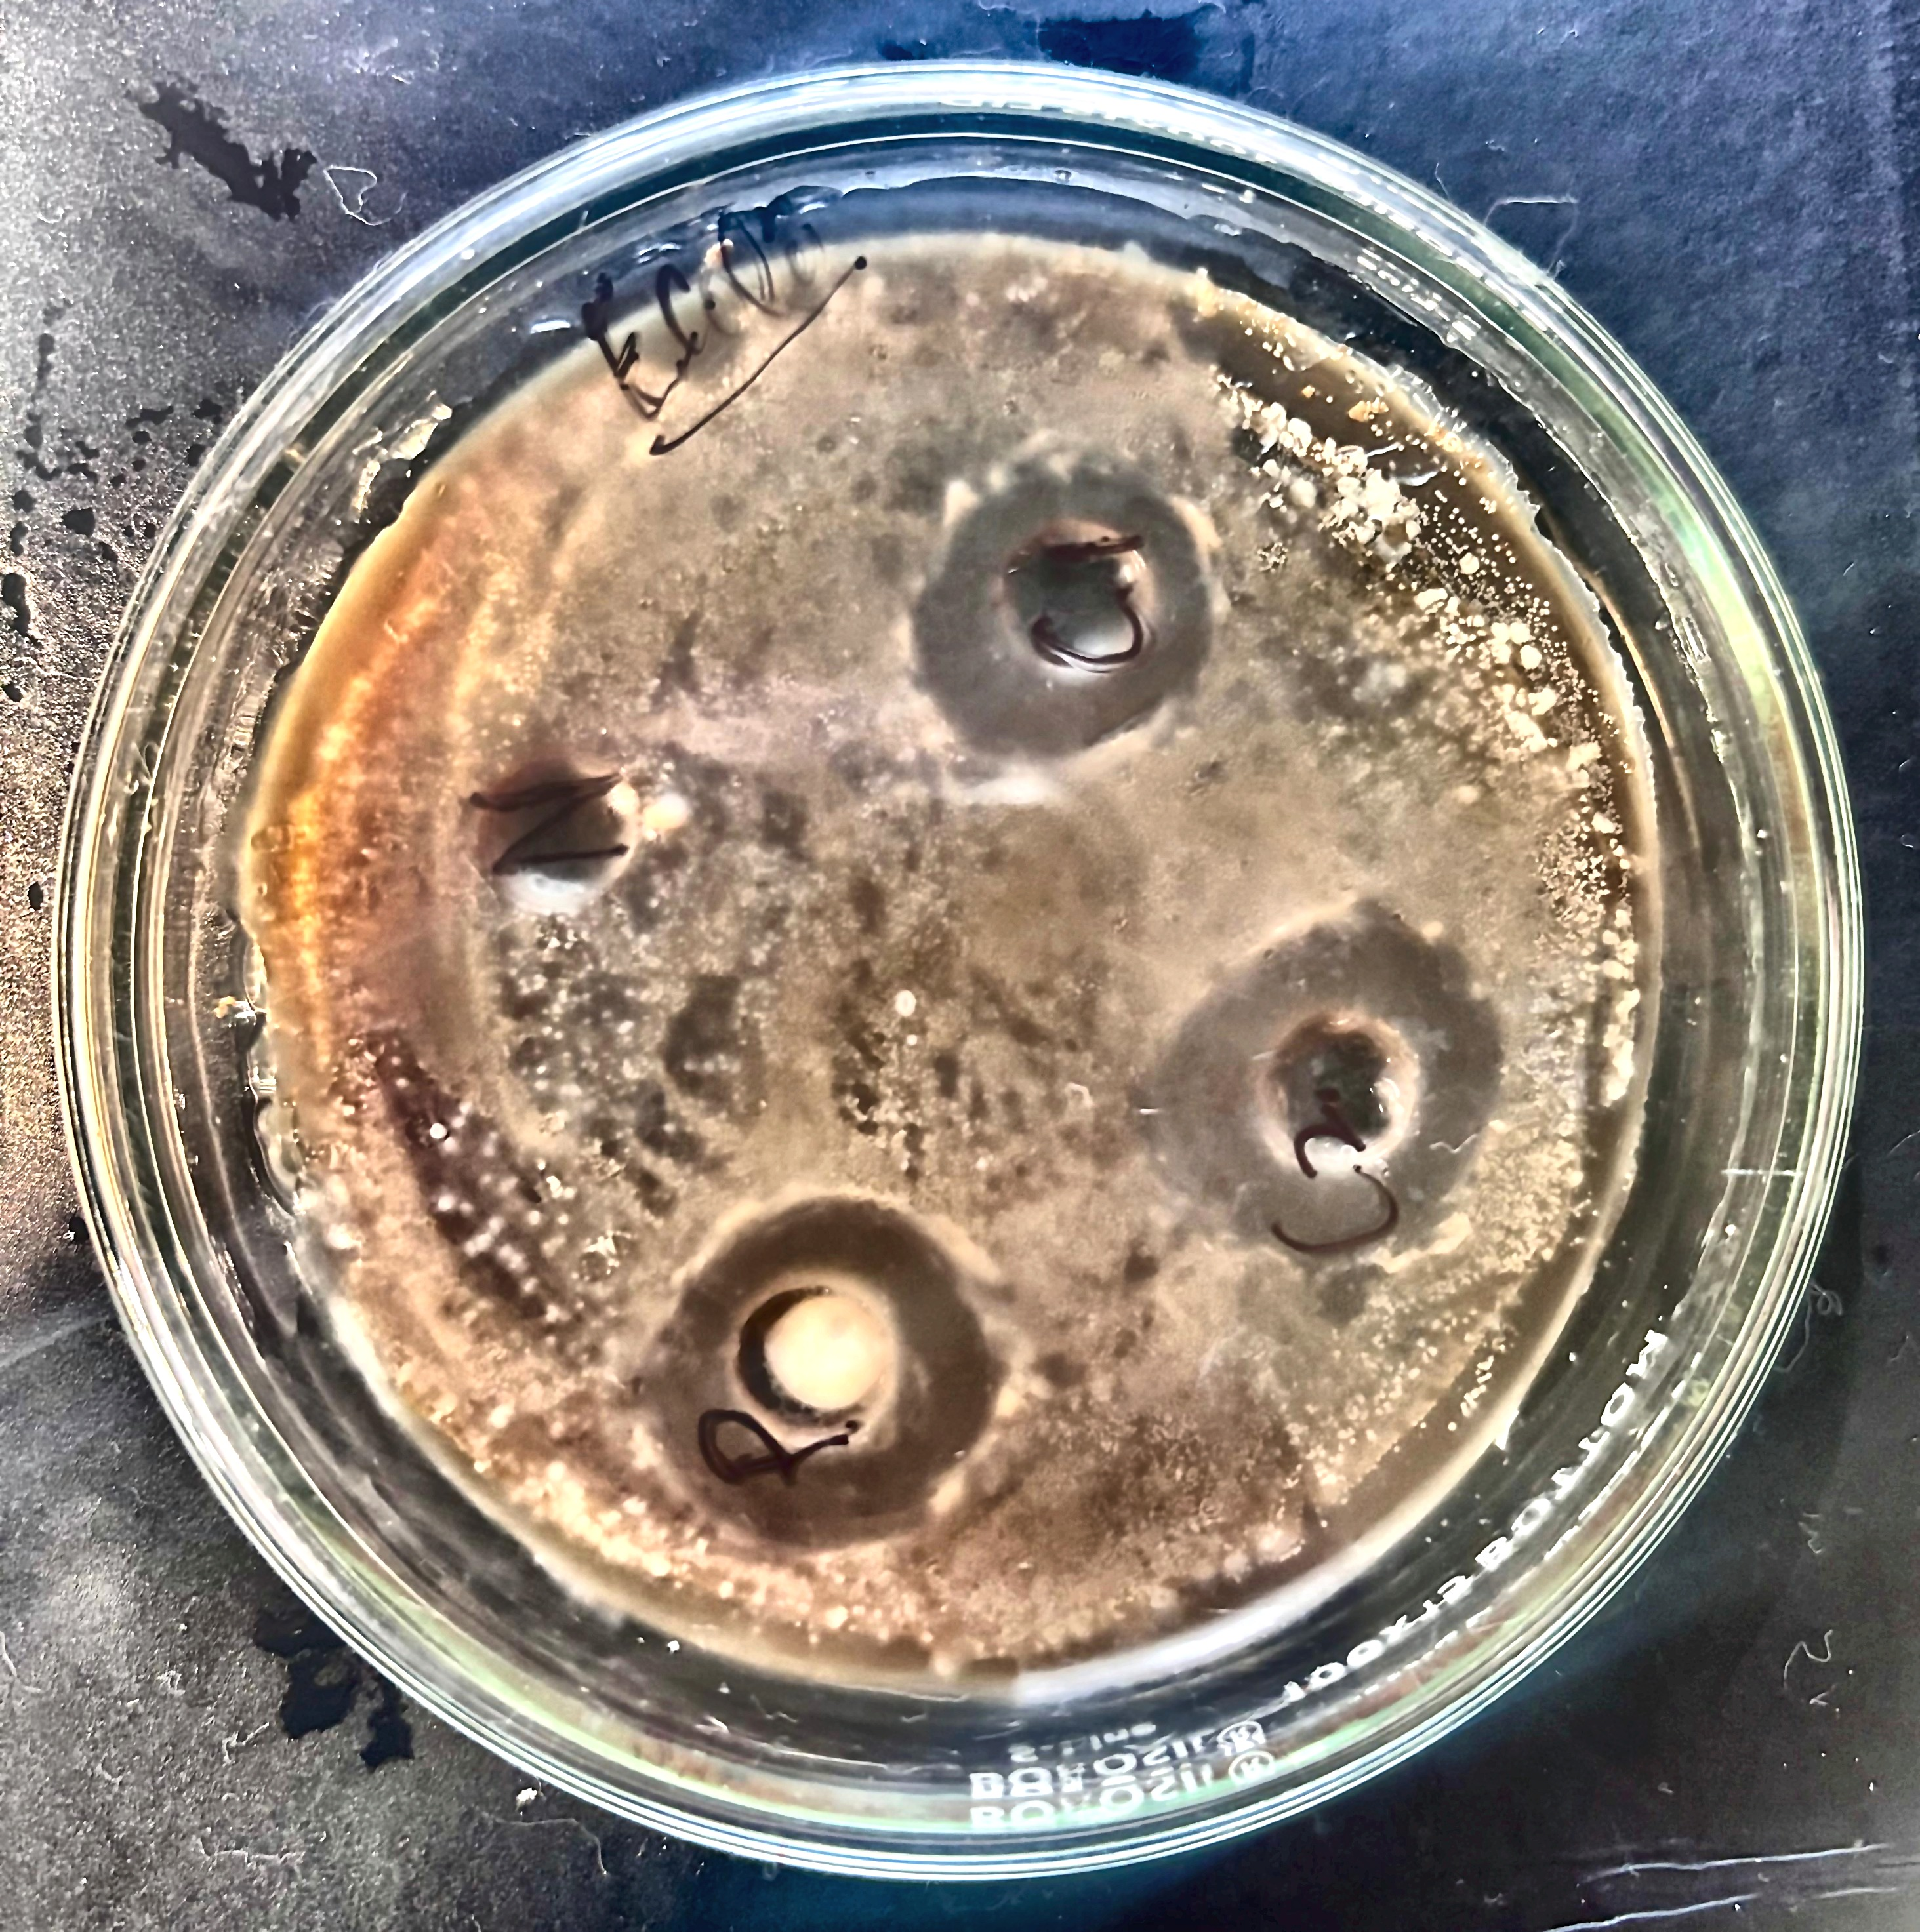
\includegraphics[width=0.72\textwidth]{figures/fig8a_ecoli_inhibition.jpg}
  \caption{Disc diffusion of aqueous \textit{D.\ inermis} against \textit{E.\ coli}. N = negative control; C = extract (C1/C2 not distinguished on the lid).}
  \label{fig:ecoli_inhibition}
\end{figure}

\section{Zone of inhibition: \textit{Pseudomonas aeruginosa}}
\label{subsec:results_paeruginosa}

Against \textit{P.\ aeruginosa}, the C1 mean ($16.03 \pm 0.25$\,mm) exceeded the C2 mean ($12.53 \pm 0.45$\,mm) (\autoref{tab:zoi_paeruginosa}). That inverse concentration pattern is reported as measured; it is not interpreted as a larger dose being more active. No inhibition photograph of \textit{P.\ aeruginosa} was available (culture plates only). The gentamicin disc mean was $17.17 \pm 0.29$\,mm. Distilled-water controls were 0.00\,mm.

\begin{table}[htbp]
  \centering
  \caption{Zone of inhibition (mm), inclusive of the disc, of aqueous \textit{D.\ inermis} against \textit{Pseudomonas aeruginosa} (mean $\pm$ SD, $n = 3$). C1 = \qty{50}{\milli\gram\per\milli\litre}; C2 = \qty{100}{\milli\gram\per\milli\litre}.}
  \label{tab:zoi_paeruginosa}
  \begin{tabular}{lcccc}
    \toprule
    Treatment & R1 & R2 & R3 & Mean $\pm$ SD \\
    \midrule
    C1 & 16.00 & 16.30 & 15.80 & $16.03 \pm 0.25$ \\
    C2 & 13.00 & 12.50 & 12.10 & $12.53 \pm 0.45$ \\
    Gentamicin disc ($+$) & 17.50 & 17.00 & 17.00 & $17.17 \pm 0.29$ \\
    Distilled water ($-$) & 0.00 & 0.00 & 0.00 & $0.00 \pm 0.00$ \\
    \bottomrule
  \end{tabular}
\end{table}

\section{Zone of inhibition: \textit{Klebsiella pneumoniae}}
\label{subsec:results_kpneumoniae}

Against \textit{K.\ pneumoniae}, C2 ($13.25 \pm 0.43$\,mm) was slightly larger than C1 ($12.35 \pm 0.56$\,mm) (\autoref{tab:zoi_kpneumoniae}; \autoref{fig:kpneumoniae_inhibition}). Gentamicin was $15.17 \pm 0.29$\,mm. Distilled-water controls were 0.00\,mm. \citet{drakhshaan2026} did not test this species. No indexed report of \textit{D.\ inermis} against \textit{K.\ pneumoniae} was located in the literature search supporting this dissertation; that is a gap in indexed sources, not a claim of absolute priority.

\begin{table}[htbp]
  \centering
  \caption{Zone of inhibition (mm), inclusive of the disc, of aqueous \textit{D.\ inermis} against \textit{Klebsiella pneumoniae} (mean $\pm$ SD, $n = 3$). C1 = \qty{50}{\milli\gram\per\milli\litre}; C2 = \qty{100}{\milli\gram\per\milli\litre}.}
  \label{tab:zoi_kpneumoniae}
  \begin{tabular}{lcccc}
    \toprule
    Treatment & R1 & R2 & R3 & Mean $\pm$ SD \\
    \midrule
    C1 & 12.00 & 13.00 & 12.05 & $12.35 \pm 0.56$ \\
    C2 & 13.50 & 13.50 & 12.75 & $13.25 \pm 0.43$ \\
    Gentamicin disc ($+$) & 15.50 & 15.00 & 15.00 & $15.17 \pm 0.29$ \\
    Distilled water ($-$) & 0.00 & 0.00 & 0.00 & $0.00 \pm 0.00$ \\
    \bottomrule
  \end{tabular}
\end{table}

\begin{figure}[htbp]
  \centering
  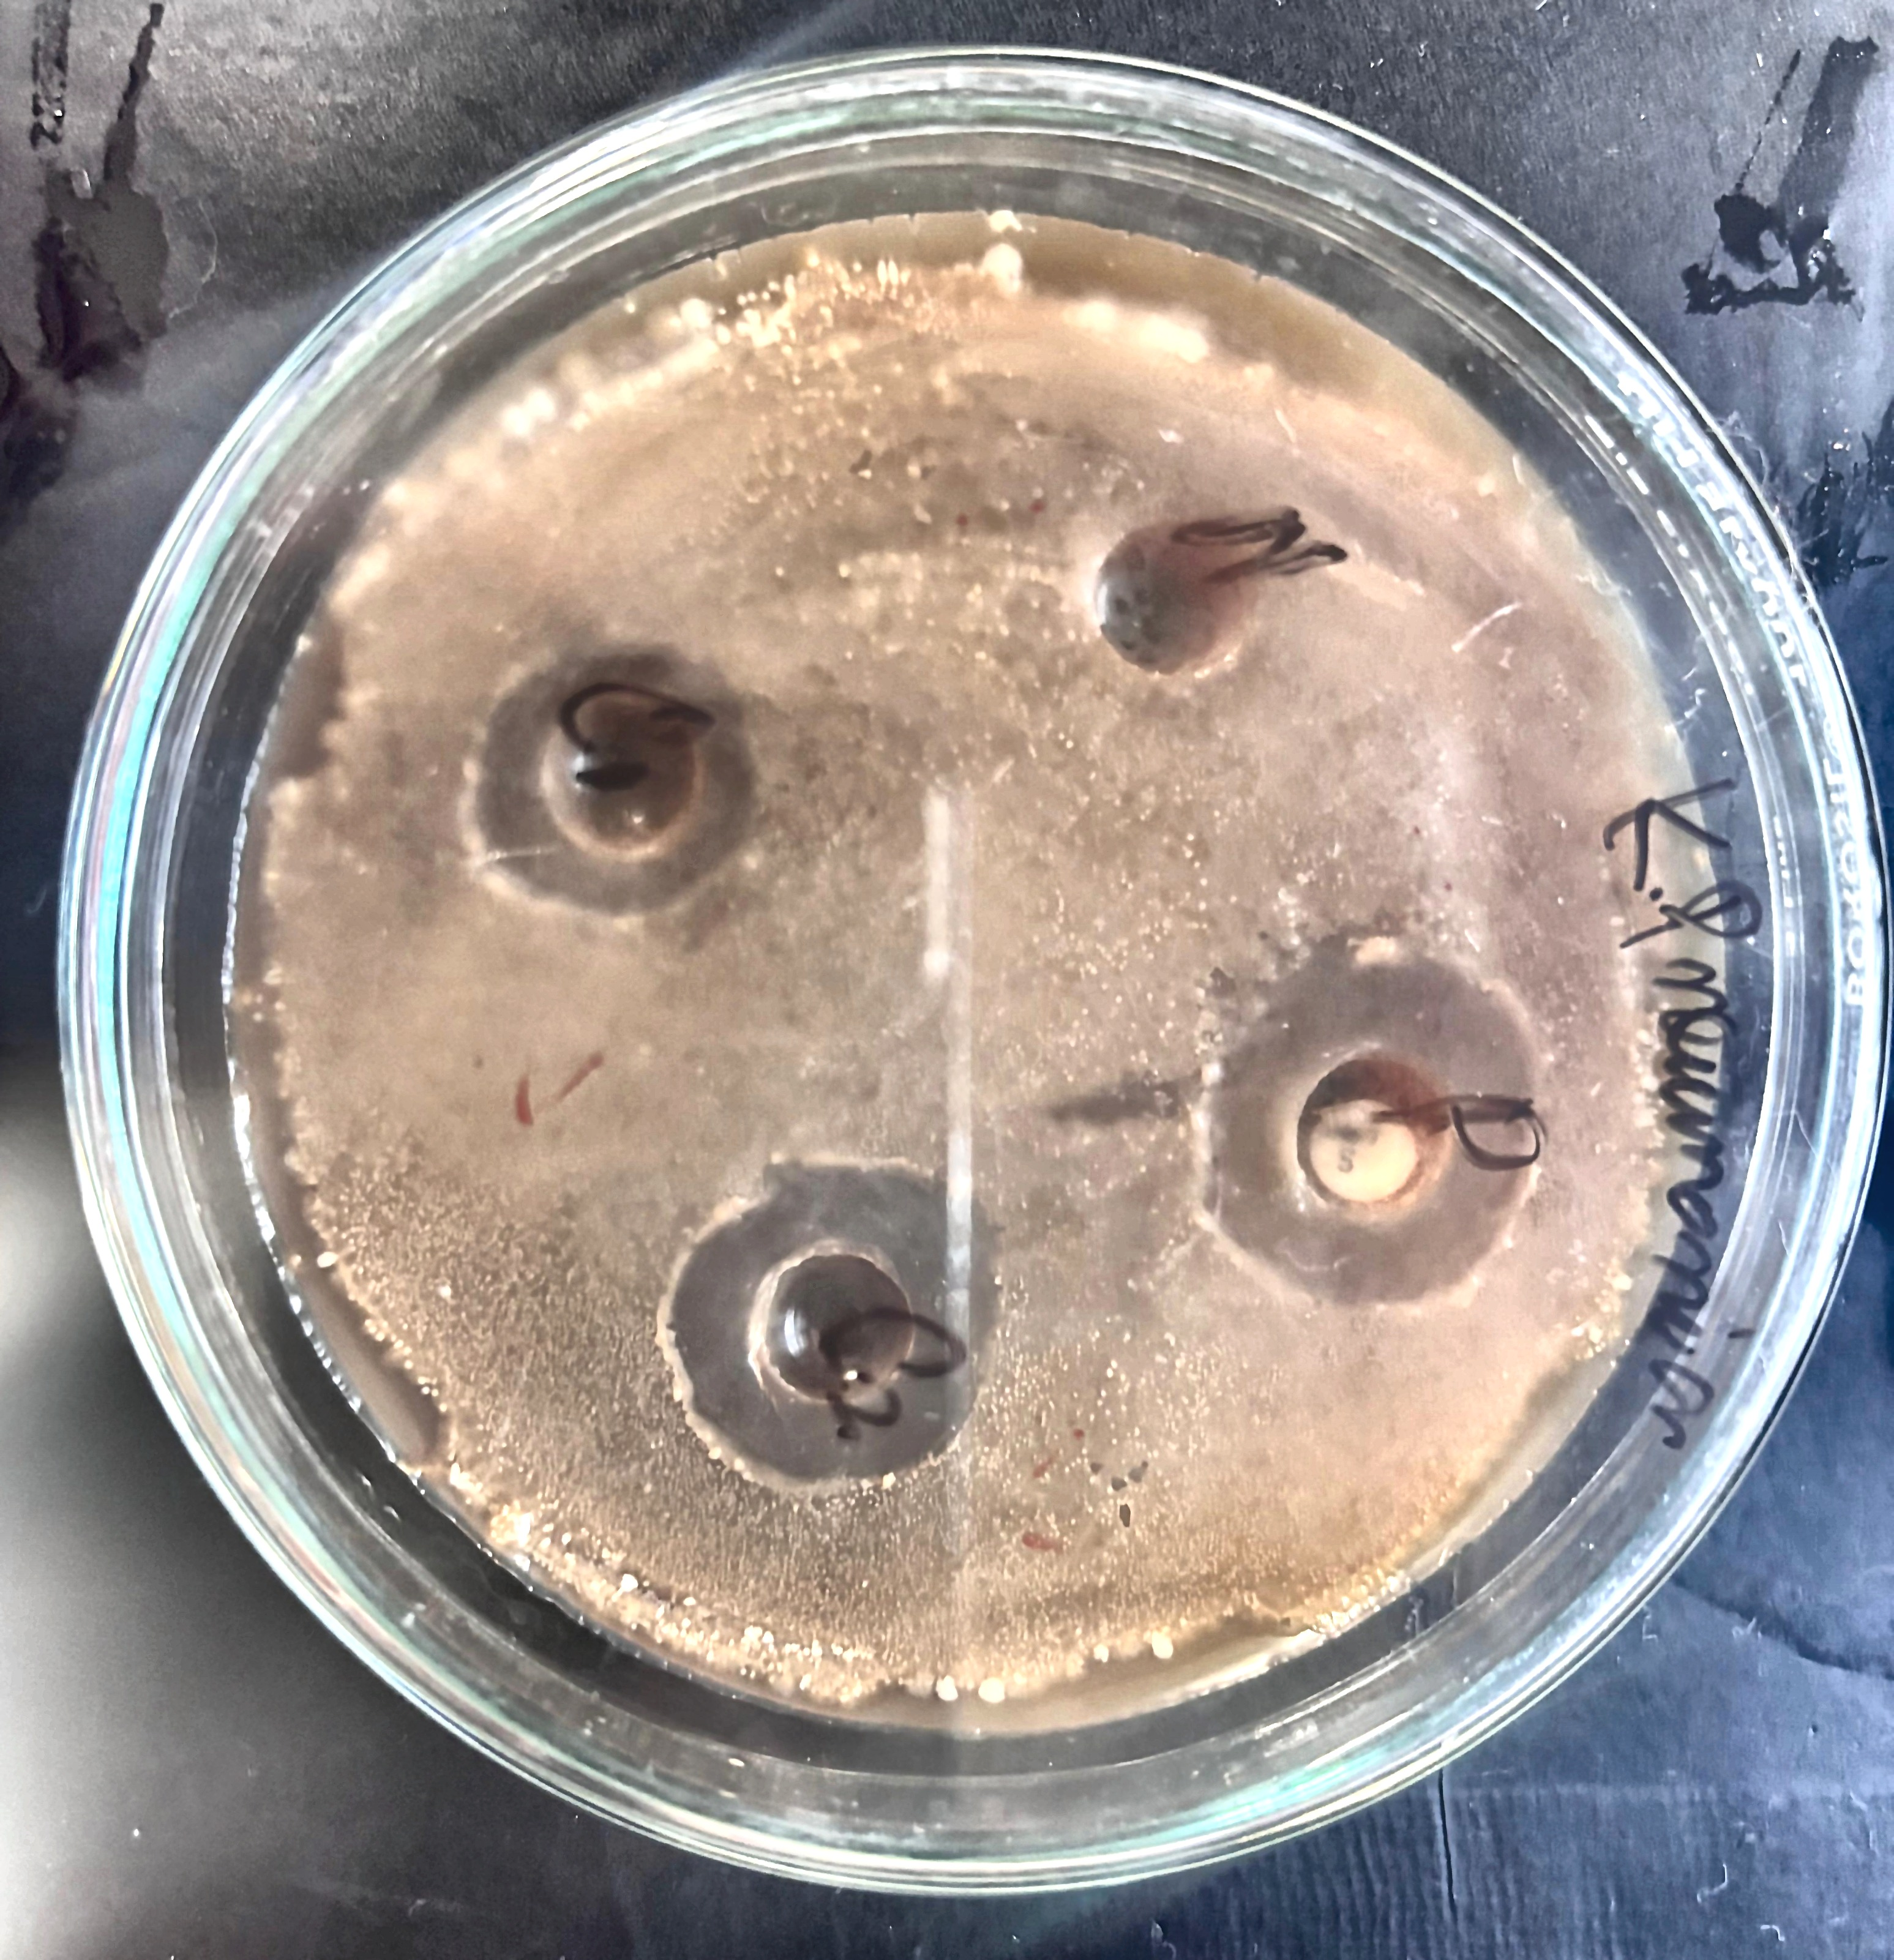
\includegraphics[width=0.72\textwidth]{figures/fig8b_kpneumoniae_inhibition.jpg}
  \caption{Disc diffusion against \textit{K.\ pneumoniae}. N = negative control; C = extract.}
  \label{fig:kpneumoniae_inhibition}
\end{figure}

\section{Comparative summary}
\label{sec:results_comparative}

\autoref{tab:zoi_comparative} places the three species together. Rank order of extract means is not the same at C1 and C2: at C1, \textit{P.\ aeruginosa} gave the largest extract zone; at C2, \textit{E.\ coli} did. Water controls were uniformly zero. Gentamicin zones were larger than the corresponding extract zones for every species.

\begin{table}[htbp]
  \centering
  \caption{Comparative zones of inhibition (mm, mean $\pm$ SD, $n = 3$).}
  \label{tab:zoi_comparative}
  \begin{tabularx}{\textwidth}{lXXXX}
    \toprule
    \textbf{Organism} & \textbf{C1} & \textbf{C2} & \textbf{Gentamicin disc} & \textbf{Water} \\
    \midrule
    \textit{E.\ coli} & $11.94 \pm 0.14$ & $14.99 \pm 0.51$ & $17.00 \pm 0.00$ & $0.00 \pm 0.00$ \\
    \textit{P.\ aeruginosa} & $16.03 \pm 0.25$ & $12.53 \pm 0.45$ & $17.17 \pm 0.29$ & $0.00 \pm 0.00$ \\
    \textit{K.\ pneumoniae} & $12.35 \pm 0.56$ & $13.25 \pm 0.43$ & $15.17 \pm 0.29$ & $0.00 \pm 0.00$ \\
    \bottomrule
  \end{tabularx}
\end{table}

\section{Comparison with published zones}
\label{sec:results_benchmarking}

\autoref{tab:organic_comparison} places C1 and C2 of this aqueous extract beside the dichloromethane and methanol well-diffusion values of \citet{drakhshaan2026} at 50 and 100\,\textmu g\,mL$^{-1}$ for the two shared species. Media, inocula, and extraction chemistry differ, so the table is a literature orientation, not a matched bioassay.

\begin{table}[hbt!]
  \centering
  \small
  \caption{Aqueous C1 and C2 (this study) versus published dichloromethane and methanol zones \citep{drakhshaan2026}. Values are mm, mean $\pm$ SD.}
  \label{tab:organic_comparison}
  \begin{tabularx}{\textwidth}{lXX}
    \toprule
    \textbf{Extract} & \textbf{\textit{E.\ coli}} & \textbf{\textit{P.\ aeruginosa}} \\
    \midrule
    Aqueous C1, this study & $11.94 \pm 0.14$ & $16.03 \pm 0.25$ \\
    Aqueous C2, this study & $14.99 \pm 0.51$ & $12.53 \pm 0.45$ \\
    DCM, 50\,\textmu g\,mL$^{-1}$ \citep{drakhshaan2026} & $12.93 \pm 0.11$ & $13.10 \pm 0.17$ \\
    DCM, 100\,\textmu g\,mL$^{-1}$ \citep{drakhshaan2026} & $15.93 \pm 0.11$ & $16.83 \pm 0.29$ \\
    MeOH, 50\,\textmu g\,mL$^{-1}$ \citep{drakhshaan2026} & $11.13 \pm 0.23$ & $9.07 \pm 0.11$ \\
    MeOH, 100\,\textmu g\,mL$^{-1}$ \citep{drakhshaan2026} & $15.80 \pm 0.34$ & $15.17 \pm 0.29$ \\
    \bottomrule
  \end{tabularx}
\end{table}

\section{Graphical summary}
\label{sec:results_graph}

\autoref{fig:zoi_barchart} plots the triplicate means and standard deviations from the laboratory table. Negative-control bars are omitted because they are zero.

\begin{figure}[hbt!]
  \centering
  \begin{tikzpicture}
    \begin{axis}[
      ybar,
      bar width=8pt,
      width=0.98\textwidth,
      height=8.4cm,
      ylabel={Zone of inhibition (mm, mean $\pm$ SD)},
      xmin=0.4, xmax=3.6,
      xtick={1,2,3},
      xticklabels={\textit{E.\ coli}, \textit{P.\ aeruginosa}, \textit{K.\ pneumoniae}},
      ymin=0, ymax=22,
      ytick={0,2,4,6,8,10,12,14,16,18,20},
      legend style={
        at={(0.5,1.05)},
        anchor=south,
        legend columns=3,
        font=\footnotesize,
        draw=none,
        /tikz/every even column/.append style={column sep=0.6em}
      },
      error bars/y dir=both,
      error bars/y explicit,
      error bars/error bar style={black, line width=0.5pt},
      grid=major,
      major grid style={gray!22},
      enlarge x limits=0.18,
    ]
      \addplot+[fill=dissertationblue!40, draw=black] coordinates {
        (1, 11.94) +- (0, 0.14)
        (2, 16.03) +- (0, 0.25)
        (3, 12.35) +- (0, 0.56)
      };
      \addplot+[fill=dissertationblue!80, draw=black] coordinates {
        (1, 14.99) +- (0, 0.51)
        (2, 12.53) +- (0, 0.45)
        (3, 13.25) +- (0, 0.43)
      };
      \addplot+[fill=dissertationgreen!70, draw=black] coordinates {
        (1, 17.00) +- (0, 0.00)
        (2, 17.17) +- (0, 0.29)
        (3, 15.17) +- (0, 0.29)
      };
      \legend{C1 (50\,mg\,mL$^{-1}$), C2 (100\,mg\,mL$^{-1}$), Gentamicin disc}
    \end{axis}
  \end{tikzpicture}
  \caption{Mean zone of inhibition (mm) for C1, C2, and the gentamicin disc. Error bars are standard deviations from the laboratory triplicates (\autoref{tab:zoi_comparative}).}
  \label{fig:zoi_barchart}
\end{figure}
